\documentclass[aspectratio=169,11pt]{beamer}

\usepackage{graphicx}
\usepackage{tikz}
\usetikzlibrary{positioning,arrows.meta}
\usepackage{xcolor}
\usepackage{booktabs}
\usepackage{tabularx}
\usepackage{array}
\usepackage{ragged2e}          

\definecolor{GEUBlue}{RGB}{20,55,105}
\definecolor{GEULightBlue}{RGB}{238,244,251}
\definecolor{GEUGrey}{RGB}{90,90,90}
\definecolor{GEULightGrey}{RGB}{245,246,248}

\usetheme{default}
\setbeamertemplate{navigation symbols}{}
\setbeamertemplate{blocks}[rounded][shadow=false]
\setbeamercolor{normal text}{fg=black,bg=white}
\setbeamercolor{frametitle}{fg=GEUBlue}
\setbeamercolor{structure}{fg=GEUBlue}
\setbeamercolor{block title}{fg=GEUBlue,bg=GEULightBlue}
\setbeamercolor{block body}{fg=black,bg=GEULightBlue}
\setbeamerfont{frametitle}{size=\Large,series=\bfseries}

% Replace with the actual logo filename
\newcommand{\GEULogo}{graphicera_logo.png}

% Header and footer
\setbeamertemplate{headline}{%
  \begin{tikzpicture}[remember picture,overlay]
    \node[anchor=north east,xshift=-0.30cm,yshift=-0.12cm]
      at (current page.north east)
      {\includegraphics[height=0.62cm]{\GEULogo}};
  \end{tikzpicture}
  \vspace{0.72cm}
}
\setbeamertemplate{frametitle}{%
  \vspace{0.03cm}
  \insertframetitle\par
  \vspace{0.04cm}
  \textcolor{GEUBlue}{\rule{\textwidth}{0.9pt}}
  \vspace{0.03cm}
}
\setbeamertemplate{footline}{%
  \leavevmode
  \hbox{%
  \begin{beamercolorbox}[wd=.82\paperwidth,ht=0.32cm,dp=0.10cm,leftskip=.3cm]{author in head/foot}
    \tiny Department of Computer Science \& Engineering | Graphic Era (Deemed to be University)
  \end{beamercolorbox}%
  \begin{beamercolorbox}[wd=.18\paperwidth,ht=0.32cm,dp=0.10cm,rightskip=.3cm]{date in head/foot}
    \hfill\tiny\insertframenumber/\inserttotalframenumber
  \end{beamercolorbox}}
}

\newcommand{\smallnote}[1]{\vspace{0.08cm}{\scriptsize\color{GEUGrey}#1}}
\newcommand{\placeholder}[1]{\textit{\color{GEUGrey}#1}}

\title{\textbf{Project-Based Learning}\\[2mm]\large Phase-I Evaluation}
\author{\textbf{Adaptive Network Routing and Failure Recovery Simulator}\\Team \#217 -- Glory Seekers}
\institute{Department of Computer Science \& Engineering\\Graphic Era (Deemed to be University), Dehradun}
\date{Academic Session 2026--27}

\begin{document}

%1
\begin{frame}[plain]
\begin{tikzpicture}[remember picture,overlay]
\draw[GEUBlue,line width=3pt] (current page.north west) -- (current page.north east);
\node[anchor=north east,xshift=-0.45cm,yshift=-0.35cm] at (current page.north east)
{\IfFileExists{\GEULogo}{\includegraphics[height=1.0cm]{\GEULogo}}{}};
\node[align=center,text width=.84\paperwidth] at ([yshift=.25cm]current page.center)
{{\color{GEUBlue}\fontsize{26}{30}\selectfont\bfseries PROJECT-BASED LEARNING}\\[3mm]
 {\fontsize{18}{22}\selectfont PHASE-I EVALUATION}\\[7mm]
 {\color{GEUGrey}\Large\bfseries \placeholder{Adaptive Network Routing and Failure Recovery Simulator}}\\[3mm]
 {\color{GEUBlue}\normalsize Team ID: 217}};
\node[align=center,anchor=south,yshift=.42cm] at (current page.south)
{\bfseries Department of Computer Science \& Engineering\\
Graphic Era (Deemed to be University), Dehradun\\[-1mm]
\scriptsize Academic Session 2026--27};
\end{tikzpicture}
\end{frame}

% 2
\begin{frame}{Team \& Mentor Details}
\begin{columns}[T,totalwidth=\textwidth]
\column{.48\textwidth}
\begin{block}{Team Information}
\begin{tabular}{@{}ll@{}}
\textbf{Team ID:} & 217\\
\textbf{Semester:} & 3rd\\
\textbf{Section:} & C,D,E,Cyber\\
\textbf{Domain:} & \placeholder{Computer Science}
\end{tabular}
\end{block}
\column{.48\textwidth}
\begin{block}{Team Members}
1.\quad \placeholder{Utkarsh Singh -- 2510012158}\\
2.\quad \placeholder{Naitik Kukreti -- 2510011904}\\
3.\quad \placeholder{Shubh Pandey -- 2510012661}\\
4.\quad \placeholder{Priyansh Bhatt -- 2510012333}
\end{block}
\end{columns}
\vspace{2mm}
\begin{block}{Mentor}
\placeholder{Ms. KumKum}
\hfill
\textbf{Interactions completed: 3}
\end{block}
\end{frame}

%3\begin{frame}{Problem Statement \& Motivation}
\begin{block}{Problem Statement}
\small
Modern computing systems depend heavily on networks for data transmission,
but network links and routers may become unavailable because of failures or
changing network conditions. When a component on a packet's route fails,
packets may be delayed, lost, or unable to reach their destination. A route
that initially works well can also become unstable after a failure or increase
in load. Therefore, network reliability requires not only finding a path, but
also maintaining communication when conditions change.
\end{block}

\vspace{0mm}

\begin{columns}[T,onlytextwidth]

\column{.48\textwidth}
\footnotesize
\textbf{\color{GEUBlue}Motivation}

\begin{itemize}
\setlength{\itemsep}{0pt}
\setlength{\parskip}{0pt}
\setlength{\parsep}{0pt}

\item \placeholder{Fixed or non-context-aware recovery strategies}
\item \placeholder{Improves network reliability by testing failures and recovery methods.}
\item \placeholder{Existing approaches use fixed recovery methods that may not suit every failure situation.}
\end{itemize}


\column{.48\textwidth}
\footnotesize
\textbf{\color{GEUBlue}Target Users / Stakeholders}

\begin{itemize}
\setlength{\itemsep}{0pt}
\setlength{\parskip}{0pt}
\setlength{\parsep}{0pt}

\item \placeholder{Students and researchers learning network routing, failures, and recovery strategies.}
\item \placeholder{Educational institutions and organizations interested in network reliability and failure management.}
\item \placeholder{A safe environment to simulate failures, compare recovery methods, and improve reliability.}
\end{itemize}

\end{columns}
% 4. OBJECTIVES
% =========================================================
\begin{frame}{Objectives}

\footnotesize

\textbf{\color{GEUBlue}Project Objectives}

\vspace{1mm}

\begin{enumerate}
\setlength{\itemsep}{1pt}
\setlength{\parskip}{0pt}
\setlength{\parsep}{0pt}

  \item \placeholder{Develop a network simulation system that detects network failures and dynamically selects an appropriate recovery strategy for reliable packet routing.}

  \item \placeholder{Implement core functionalities including network topology creation, packet routing, failure simulation, and adaptive recovery strategy selection.}

  \item \placeholder{Integrate Data Structures in C and Object-Oriented Programming in C++ concepts for efficient network modeling, routing, and failure recovery.}

  \item \placeholder{Evaluate the system using packet delivery, packet loss, path cost, and recovery time under different failure scenarios.}

  \item \placeholder{Demonstrate the practical use of adaptive network recovery and explore future enhancements for real-world network resilience.}

\end{enumerate}

\vspace{2mm}

\begin{center}
\colorbox{GEULightBlue}{
\parbox{.85\textwidth}{
\centering
\textbf{Key Objective:}
\placeholder{To Develop and evaluate a network simulator that improves failure recovery by dynamically selecting suitable recovery strategies based on network conditions.}
}}
\end{center}

\end{frame}

% 5
\begin{frame}{Proposed Solution}

\small

\begin{tabular}{p{0.35\textwidth} p{0.55\textwidth}}

\textbf{\color{GEUBlue}Proposed Approach} &
\textbf{\color{GEUBlue}Key Features} \\[3mm]

1. \placeholder{Input / Data Collection} &
\placeholder{Accepts network topology and failure scenarios as simulation input.} \\[3mm]

2. \placeholder{Processing / Core Algorithm} &
\placeholder{Uses routing algorithms and selects appropriate recovery strategies.} \\[3mm]

3. \placeholder{System Logic} &
\placeholder{Analyzes network conditions to determine routing or recovery actions.} \\[3mm]

4. \placeholder{Database / Storage} &
\placeholder{Stores network configurations, simulation events, and results.} \\[3mm]

5. \placeholder{Output / Visualization} &
\placeholder{Displays routing paths, recovery actions, and performance results.}

\end{tabular}

\end{frame}
% 6
\begin{frame}{Integration of PBL Course Concepts}

\scriptsize

\begin{center}
\renewcommand{\arraystretch}{1.25}

\begin{tabularx}{.96\textwidth}{@{}>{\bfseries}p{3.0cm}X p{3.0cm}@{}}
\toprule
Course & Concepts Applied & Project Module\\
\midrule

Data Structures in C &
Graphs for network representation; linked lists for dynamically changing
connections/paths; queues for efficient selection; hash tables for fast lookup &
Network representation and routing \\

OOPs with C++ &
Classes, encapsulation, inheritance and polymorphism for modelling routers,
links and packets &
Network simulation objects \\

\bottomrule
\end{tabularx}

\end{center}

\vspace{4mm}

\begin{block}{Meaningful Integration}
The project combines graph and other data-structure concepts with C++ object-oriented
design to create a network simulator. Graphs model topology, while classes model
network entities such as routers, links and packets.
\end{block}

\vfill

\begin{center}
\end{center}

\end{frame}

% 7
\begin{frame}{System Architecture / Workflow}
\begin{center}
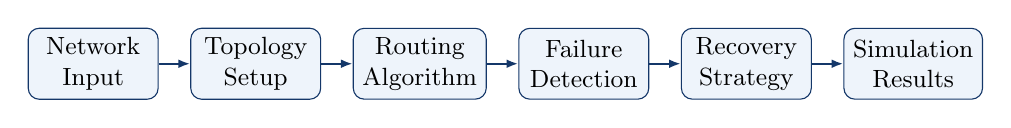
\begin{tikzpicture}[
node distance=4mm,
box/.style={
    rectangle,
    rounded corners,
    draw=GEUBlue,
    fill=GEULightBlue,
    minimum width=1.65cm,
    minimum height=9mm,
    align=center,
    font=\small
},
arrow/.style={-{Latex[length=1.5mm]},thick,draw=GEUBlue}
]

\node[box] (a) {Network\\Input};
\node[box,right=of a] (b) {Topology\\Setup};
\node[box,right=of b] (c) {Routing\\Algorithm};
\node[box,right=of c] (d) {Failure\\Detection};
\node[box,right=of d] (e) {Recovery\\Strategy};
\node[box,right=of e] (f) {Simulation\\Results};

\draw[arrow] (a)--(b);
\draw[arrow] (b)--(c);
\draw[arrow] (c)--(d);
\draw[arrow] (d)--(e);
\draw[arrow] (e)--(f);


\end{tikzpicture}
\end{center}
\vspace{5mm}
\begin{columns}[T,totalwidth=\textwidth]
\column{.48\textwidth}
\textbf{\color{GEUBlue}Major Components}
\begin{itemize}\itemsep2pt
\item \placeholder{Network Topology & Graph}
\item \placeholder{Routing & Packet Management}
\item \placeholder{Failure Detection & Recovery}
\end{itemize}
\column{.48\textwidth}
\textbf{\color{GEUBlue}Data / Control Flow}
\begin{itemize}\itemsep2pt
\item \placeholder{Network topology and packets are provided as input}
\item \placeholder{Routing algorithm selects the initial path}
\item \placeholder{Failures trigger detection and recovery mechanisms}
\end{itemize}
\end{columns}
\end{frame}

% =========================================================
% 8. TECHNOLOGY STACK & METHODOLOGY
% =========================================================
\begin{frame}{Technology Stack \& Methodology}

\begin{columns}[T,onlytextwidth]

% LEFT COLUMN
\column{.47\textwidth}

\begin{block}{Technology Stack}
\footnotesize

\begin{itemize}
\setlength{\itemsep}{1pt}

  \item Programming: C / C++
  \item Development Environment: Visual Studio Code
  \item Data Structures: Graphs, Linked Lists, Queues, Hash Tables
  \item UI: Project Interface / Visualization
  \item Version Control: Git / GitHub

\end{itemize}
\end{block}


% RIGHT COLUMN
\column{.49\textwidth}

\begin{block}{Development Methodology}
\footnotesize

\begin{enumerate}
\setlength{\itemsep}{1pt}

  \item Identify project requirements, inputs, and outputs.
  
  \item Design the network topology, routing, packet, and recovery modules.
  
  \item Develop the simulator using C++ and data structures.
  
  \item Simulate network failures and test recovery mechanisms.
  
  \item Evaluate packet delivery, loss, path cost, and recovery time.

\end{enumerate}
\end{block}

\end{columns}

\vspace{1mm}

\begin{center}
\scriptsize
\smallnote{C/C++ supports efficient implementation of data structures,
graph algorithms, and object-oriented network entities.}
\end{center}

\end{frame}

% =========================================================
% 9. INITIAL PROGRESS & TEAM CONTRIBUTION
% =========================================================
\begin{frame}{Initial Progress \& Team Contribution}

\begin{columns}[T,onlytextwidth]

% LEFT COLUMN
\column{.45\textwidth}

\footnotesize
\textbf{\color{GEUBlue}Progress Achieved}

\begin{itemize}
\setlength{\itemsep}{1pt}

  \item Project problem and motivation identified.
  \item Routing and recovery approaches studied.
  \item Network model and architecture planned.
  \item Required data structures and OOP concepts identified.
  \item Routing, failure simulation, and recovery workflow defined.
  \item Evaluation parameters identified.

\end{itemize}


% RIGHT COLUMN
\column{.50\textwidth}

\footnotesize
\textbf{\color{GEUBlue}Individual Contribution}

\vspace{1mm}

\scriptsize

\begin{tabularx}{\linewidth}{@{}p{1.25cm}p{1.25cm}X@{}}
\toprule
Member & Role & Contribution\\
\midrule

Utkarsh & Team Lead & Coordination and project planning\\
Naitik & Member & Project design and implementation support\\
Shubh & Member & Data structures and algorithm support\\
Priyansh & Member & C/C++ development and UI support\\

\bottomrule
\end{tabularx}

\vspace{1mm}

\scriptsize
\textit{Note: Member responsibilities are kept at a general project level.}

\end{columns}

\end{frame}

% =========================================================
% 10. ROADMAP, OUTCOMES & REFERENCES
% =========================================================
\begin{frame}{Roadmap, Expected Outcomes \& References}

\footnotesize

\begin{columns}[T,onlytextwidth]

\column{.48\textwidth}

\textbf{\color{GEUBlue}Roadmap}

\begin{enumerate}
\setlength{\itemsep}{1pt}
\item Phase-I: Proposal \& Design
\item Phase-II: Development
\item Phase-III: Final Implementation
\end{enumerate}

\vspace{1mm}

\textbf{\color{GEUBlue}Expected Outcomes}

\begin{itemize}
\setlength{\itemsep}{1pt}
\item Working network simulator
\item Router, link, packet, and topology model
\item Routing and alternate-route recovery
\item Adaptive recovery selection
\item Performance comparison using key metrics
\end{itemize}


\column{.48\textwidth}

\textbf{\color{GEUBlue}References}

\begin{enumerate}
\setlength{\itemsep}{2pt}
\item GeeksforGeeks -- Graph Data Structure
\item GeeksforGeeks -- Dijkstra's Algorithm
\item RFC 2328 -- OSPF Version 2
\item RFC 5880 -- BFD
\end{enumerate}

\vspace{3mm}

\begin{center}
\colorbox{GEUBlue}{%
\parbox{.75\linewidth}{%
\centering
\color{white}\textbf{Thank You}\\
Questions \& Suggestions
}}
\end{center}

\end{columns}

\end{frame}

\end{document}